\chapter{State of the Art for IEEE 802.11 Power Save}

The power save algorithm described in this thesis is implemented starting from the classical power save algorithm implemented in the ath9k_htc driver with direct applicability to the AR9271 chip.

In this chapter I present the AR9271 chipset and the interaction between mac80211, ath9k_htc driver and AR9271 firmware with emphasis on the power save mechanism.

\section{AR9271 Chip}
\label{sec:chip}

As stated in the datasheet, the Atheros AR9271 is a highly integrated single-chip solution for 2.4 GHz 802.11n-ready wireless local area networks (WLANs) that enables a high-performance 1x1 configuration for wireless station applications demanding robust link quality and maximum throughput and range. The AR9271 integrates a multi-protocol MAC, baseband processor, analog-to-digital and digital-to-analog (ADC/DAC) converters, 1x1 radio transceiver, RF switch, and USB interface in an all-CMOS device for low power and small form factor applications.

\fig[scale=0.5]{src/img/ar9271.png}{img:ar9271-overview}{AR9271 system block diagram} 

The AR9271 implements half-duplex OFDM, CCK, and DSSS baseband processing, supporting 72.2 Mbps for 20 MHz and 150 Mbps for 40 MHz channel and IEEE 802.11b/g data rates. Other features include signal detection, automatic gain control, frequency offset estimation, symbol timing, and channel estimation. The AR9271 MAC supports the 802.11 wireless MAC protocol, 802.11i security, receive and transmit filtering, error recovery, and quality of service (QoS).

The AR9271 supports one transmit traffic stream and one receive traffic stream using one integrated Tx chain and one receive chain for high throughput and range performance. The Tx chain combines baseband in-phase (I) and quadrature (Q) signals, converts them to the desired frequency, and drives the RF signal to the antenna. The frequency synthesizer supports frequencies defined by IEEE 802.11b/g/n specifications.

The AR9271 supports frame data transfer to and from the host using a USB interface that provides interrupt generation/reporting, power save, and status reporting. Other external interfaces include serial EEPROM and GPIOs. The AR9271 is interoperable with standard legacy 802.11b/g devices.

\section{IEEE802.11 Power Save}
\label{sec:powersaveieee80211}

As decribed at \cite{cite-powersavestandard}, to assist stations with power saving, Access Points (APs) are designed to buffer frames for a station when that station is in power save mode and to transmit them later to the station when the AP knows the station will listen. When a station is in power save mode, it turns off its transmitter and receiver to preserve energy. It takes less power for a station to turn its receiver on to listen to frames than to turn it its transmitter on to transmit frames. For this reason, it's more power-efficient for an AP to inform a station if it has buffered frames present on the AP than to have the station poll the AP querying if frames are present.

\subsection{Target Beacon Transmission Time Time (TBTT) and beacon interval}
\label{sub-sec:proj-tbtt}

Target Beacon Transmission Time Time (TBTT) is the time at which a node (AP or station when in Ad-hoc) must send a beacon. The time difference between two TBTTs is known as the beacon interval. The beacon interval is given in Time Units (TU), each TU represents 1024 microseconds. The beacon interval is typically set to 100 TUs (102400 microseconds, or 102.4 ms) and its length is two bytes.

During association, a “Listen Interval” field is provided by the station. The listen interval is given in beacon interval units, so essentially it tells the AP how many beacons it wants to ignore before turning the receiver on. Two bytes are used to represent he listen interval. Depending on how the AP is tuned, usually based on the amount of space desired for buffered frames, the association may or may not be rejected. After the listen interval the AP does not guarantee it will buffer frames for the station anymore and may discard them. As might be expected then, the listen interval can be used by the AP as a guaranteed maximum time before stations listen to one of their beacons.

\subsection{The TIM information element}
\label{sub-sec:proj-timinfoelement}

The IEEE-802.11 standards chose to use a bitmap to indicate to any sleeping listening stations if the AP has any buffered frames present for it. Because stations should listen to at least one beacon before the listen interval, the AP periodically sends this bitmap on its beacons as an information element. The bitmask is called the Traffic Indication Map and consists of 2008 bits, each bit representing the Association Id (AID) of a station. For example, the TIM information element allows you to transfer 1 byte up to the entire 251 bytes (2008 bits) of the TIM. You are allowed to transmit a smaller TIM bitmap as it is expected that only a few number of stations will be asleep. Because of this the bitmap values passed in the TIM information element is called a partial virtual bitmap. To allow you to transmit only a partial bitmap you must make use of the bitmap control and length fields of the TIM information element.

\subsection{Retrieving buffered unicast frames}
\label{sub-sec:proj-buffered}

After a station receives a TIM and if its sees that the AP has buffered frames for it, it must send a Power Save Poll (NULL frame with Power Save Bit Set) control frame to retrieve each buffered frame on the AP. A station may go back to sleep after the PS-Poll ↔ frame exchange or once the TIM no longer has its AID present.

\subsection{Delivery Traffic Indication Map (DTIM), DTIM period}
\label{sub-sec:proj-dtim}

We use a special type of TIM to to announce that the AP is about to transmit all buffered broadcast and multicast frames called the Delivery Traffic Indication Map (DTIM). After this DTIM the AP will send all buffered broadcast and multicast frames. The DTIM will be sent every DTIM period. The DTIM period is set on the TIM information element on the DTIM period field. This field is one byte and represents the number of beacon intervals that must go by before a new DTIM is sent. The DTIM count on the TIM information element tells stations how many beacons must be transmitted before receiving the next DTIM. The DTIM count will be 0 when we've reached a DTIM.

\section{mac80211 power save}
\label{sec:mac80211}
This chapter describes the main functions used by the mac80211 layer for implementing IEEE802.11 Power Save.

Important flags:
\begin{itemize}
\item IEEE80211_CONF_PS: Enable 802.11 power save mode (managed mode only). This is the standard power save mode, meaning that the hardware still wakes up for beacons, is able to transmit frames and receive the possible acknowledgment frames. Not to be confused with hardware specific wakeup/sleep states.
\item IEEE80211_CONF_CHANGE_PS: signals that the PS flag or the dynamic PS timeout changed. This flag is checked if IEEE80211_CONF_PS is set.
\item IEEE_80211_HW_SUPPORTS_PS: hardware support for power save.
\item IEEE80211_STA_NULLFUNC_ACKED: set when the NULL frame with PS bit set is ACK'ed.
\item IEEE80211_HW_REPORTS_TX_ACK_STATUS: hardware can provide ack status reports of tx frames to the stack.
\end{itemize}

Important timers:
\begin{itemize}
\item ieee80211_dynamic_ps_timer: Each time this timer expires, mac80211 will try to enable PS mode by calling ieee80211_dynamic_ps_enable_work tasklet.
\end{itemize}

Important functions:
\begin{itemize}
\item ieee80211_rx_mgmt_beacon: this function checks if the AID is set in TIM. If the card is in PS mode then it will disable PS by unsetting the IEEE80211_CONF_PS and requesting the driver to put the hardware in a low-energy mode by calling ieee80211_hw_config with IEEE80211_CONF_CHANGE_PS parameter. After that, it will send a NULL frame to the AP with the PS but unset.
\item ieee80211_dynamic_ps_enable_work tasklet: The role of this function is to trigger the PS mode. Several checks are done before entering PS mode: check if there are no pending frames to transmit and check that the sending queues are not stopped for any reason. If all these checks are passed then enter PS mode if the NULL frame previously sent is ACK'ed. Otherwise, trigger the resending of the NULL frame with PS bit set.
\item ieee80211_dynamic_ps_disable_work: This function unsets the IEEE80211_CONF_PS then wakes up the hardware by calling ieee80211_hw_config with IEEE80211_CONF_CHANGE_PS. Also, the pending frames from the queues that were stopped due to IEEE80211_QUEUE_STOP_REASON_PS are required to be processed.
\item ieee80211_rx_h_data: ieee80211_dynamic_ps_timer is rearmed.
\item ieee80211_tx_h_dynamic_ps: if the card is not in power save mode, then the ieee80211_dynamic_ps_time is re'armed. Otherwise, if the card is in PS mode, enqueue frames, unset IEEE80211_STA_NULLFUNC_ACKED, set the queue stop reason as IEEE80211_QUEUE_STOP_REASON_PS and schedule ieee80211_dynamic_ps_disable_work.
\item ieee80211_tx_status: This function sets the IEEE80211_STA_NULLFUNC_ACKED if the NULL frame with PS bit is ACK'ed. This functionality is supported only if hardware has IEEE80211_HW_REPORTS_TX_ACK_STATUS capability.
\item ieee80211_mgd_probe_ap: this functions is called when several beacons are missed. Once the station receives a beacon it will start the ieee80211_sta_bcn_mon_timer timer, initialized with a time equal with multiple of beacon intervals. The card might be in sleep mode but it still wakes up to receive beacons. If it wakes up several times at beacon interval but no beacon is received then the PS mode is disabled and the card stays on until it receives a beacon/declares the connection lost.
\end{itemize}

\section{ath9k_htc power save}
\label{sec:ath9khtc}

The main role of the ath9k_htc driver is to configure the Wi-Fi card hardware timers such that the card wakes up properly for beacons at TIM/DTIM period. The RTC subsystem is always on and can be programmed to wake up periodically the MAC subsystem (see \labelindexref{Figure}{img:ar9271-overview}). The RTC handles clock generation and power save signaling and is the only thing in the chip that stays on during power or full sleep states. MAC_PCU_SLP1 and MAC_PCU_SLP2 registers together  with NEXT_TIM, NEXT_DTIM and TBTT timers control when the AR9271 should wake when waiting for AP Rx traffic.

MAC_PCU_SLP1 register bits:
\begin{itemize}
\item CAB_TIMEOUT: Time in TU that the MAC waits for CAB after receiving the beacon or the previous
CAB, insuring that if no CAB is received after the beacon is received or if a long gap occurs between CABs, the MAC powersave state returns to idle
\item ASSUME_DTIM: A mode bit which indicates whether to assume a beacon was missed when the
SLP_BEACON_TIMEOUT: occurs with no received beacons, in which case is assumes
the DTIM was missed, and waits for CAB.
\end{itemize}

MAC_PCU_SLP2 can be configured with BEACON_TIMEOUT: Time in TU that the PCU waits for a beacon after waking up. If this time expires, the MAC woke due to SLP_NEXT_DTIM, and SLP_ASSUME_DTIM is active, then it assumes the beacon was missed and goes directly to watching for CAB. Otherwise when this time expires, the beacon powersave state returns to idle.

NEXT_TIM and NEXT_DTIM are configured with two values: when the timer should trigger for the first time and the period for that trigger.

Using these registers, ath9k_htc defines two power level: ATH9K_PM_NETWORK_SLEEP, when the card is in low power mode and ATH9K_PM_AWAKE. The main functions defined by the driver are ath9k_htc_setpower which can set the card in one of the above states, ath9k_ps_work which sets the card to ATH9K_PM_AWAKE state for a short period of time then sets its state back to ATH9K_PM_NETWORK_SLEEP.

\section{Interaction between mac80211 and ath9k_htc}
\label{sec:ath9khtcmac80211interction}

\subsection{Receive beacon with TIM unset while card is in sleep state}
\label{sub-sec:analysis-1}
ath9k_rx_tasklet: 
\begin{itemize}
\item receive a beacon, PS is enabled for the interface
\item call mac80211 callback for processing of enqueued frames
\end{itemize}
ieee80211_rx_mgmt_beacon:
\begin{itemize}
\item receive a beacon with the TIM unset - first one
\item notify the driver about beacon receive: card is put in the AWAKE state in order to set sleep registers and timers, TIM and DTIM timers are adjusted with info from the last beacon and wifi card is put back in sleep state
\end{itemize}
after beacon interval ms, hardware timers wakes up the wifi card and the process repeats

\subsection{Receive beacon with TIM set while card is in sleep state}
\label{sub-sec:analysis-2}
ath9k_rx_tasklet: 
\begin{itemize}
\item receive a beacon, PS is enabled for the interface
\item call mac80211 callback for processing of enqueued frames
\end{itemize}
ieee80211_rx_mgmt_beacon:
\begin{itemize}
\item send a notification to the driver for waking up the card
\item send NULL frame with the PS bit unset for announcing the AP that it can send the buffered frames
\end{itemize}
ieee80211_tx_h_dynamic_ps:
\begin{itemize}
\item triggered by the sending of the SKB with the NULL function: ieee80211_dynamic_ps_timer is rearmed
\end{itemize}
ieee80211_rx_h_data:
\begin{itemize}
\item triggered by the receipt of the ACK for the NULL frame: ieee80211_dynamic_ps_timer is rearmed
\end{itemize}

\subsection{Send frame and exit from sleep state}
\label{sub-sec:analysis-3}
ieee80211_tx_h_dynamic_ps:
\begin{itemize}
\item stop queues with reason IEEE80211_QUEUE_STOP_REASON_PS
\item unset IEEE80211_STA_NULLFUNC_ACKED
\item schedule ieee80211_dynamic_ps_disable_work tasklet for disabling PS
\item delay ieee80211_dynamic_ps_timer, the timer responsible for putting the card in sleep mode
\end{itemize}
ieee80211_dynamic_ps_disable_work:
\begin{itemize}
\item request driver to put the card in the awake state
\item wake queues that are sleeping with IEEE80211_QUEUE_STOP_REASON_PS
\end{itemize}
after a while, the dynamic_ps_timer expires and ieee80211_dynamic_ps_enable_work is scheduled:
\begin{itemize}
\item check that IEEE80211_STA_NULLFUNC_ACKED is unset and send NULL frame with the PS bit set
\item at this moement the card is still in the AWAKE state
\end{itemize}
ath9k_rx_tasklet->ieee80211_rx_mgmt_beacon
ieee80211_dynamic_ps_enable_work is scheduled and the card is put into sleep state

\chapter{Nexus 5 Analysis}

One of the first Android phones used for studying the Multiple Wireless Connectivity was the Google Nexus 5 \cite{cite-nexus5}. The main reason for this choice is the availability of both 2.4 Ghz and 5Ghz Wi-Fi frequencies which opens the door for the analysis of channel switching use-cases. 

The analysis is focused on the parallel usage of both the regular Wi-Fi 802.11 connectivity and Wi-Fi Direct connectivity. The main discovery is that the Power Save algorithm is automatically disabled once a second virtual interface is created, in this particular case the interface for the Wi-Fi Direct connection. 

What I tried to do was to replace this second interface with an interface for a secondary Wi-Fi 802.11 connection then implement my own Power-Save algorithm but this proved to be a show-stopper because the firmware for Nexus 5 is closed-source and it was impossible to make the stack work in parallel with two virtual interfaces in managed mode.


\section{Testbed}
\label{sec:testbed}

Some modifications had to be done to the Wi-Fi Direct functionality so CyanogenMod 13 Hammerhead was chosen as operating system as the community was very active when the work for this project was started (2014). In the meantime, the original project died and was rebranded in Lineage OS \cite{cite-lineage}.

As hardware I used an AC750 Wireless Dual Band Gigabit Router \cite{cite-router}, a Monsoon Power Monitor device \cite{cite-monsoon}, a WiFi Spectrum analyzer and two Nexus 5 smartphones. One of the phones acts as P2P-GO and the other one as P2P client. In some tests, the P2P client is also connected to the Access Point. Also, in some tests, the Power Monitor Device measures the power consumption of the P2P client.

\subsection{Capturing Air Packets}
\label{sub-sec:proj-scopemonitormode}

The first attempt to capture the packets for the Wi-Fi Direct connection was to use an Intel Dual Band Wireless-AC 7260 card \cite{cite-intel7260} in monitor mode then to use Wireshark \cite{cite-wireshark}  for analysis. The problem was that only control frames like RTS/CTS and Block ACK were captured but no data packets.

However, the Wi-Fi Spectrum analyzer (see \labelindexref{Figure}{img:chananalyzer-capture}) showed us that channel 1 was almost fully occupied so data frames were transmitted but our card in monitor mode couldn't decode those frames.

\fig[scale=0.5]{src/img/chananalyzer.jpg}{img:chananalyzer-capture}{Spectrum analyzer capture}

After starting a discussion \cite{cite-monitordiscussion} with the Intel Wi-Fi driver maintainer (iwlwifi), it proved that the problem was caused by the lack of low-density parity-check (LDPC) coding capability in hardware. Our card, Intel 7260 supports only Viterbi decoding. The next step was trying to install an Intel 7265 card which does support LDPC. The problem was that our laptop uses the older mini-PCIe connection while we needed an M.2 connection for the 7265 card.

Unable to install a newer card we tested an external card, a TP-Link TL-WN722N card \cite{cite-tplink} which proved to have LDPC capabilities. The problem with this card is the limitation to capture only 802.11n packets on the 2.4 frequency.

Wireshark was setup with the SSID and the password for the Wi-Fi Direct connection in order to decrypt the air packets. This parameters were taken from the P2P-GO and setup in Wireshark: Edit->Preferences->Protocols->IEEE 802.11->Decryption Keys->wpa pwd.

\begin{lstlisting}[language=C, frame=single, caption={Listing from /data/misc/wifi/p2p_supplicant.conf on the P2P GO},label=p2p_supplicant]
network={
	ssid="DIRECT-gQ-Android_cf8c"
	bssid=be:f5:ac:ff:e5:df
	psk="Lkb7rPop"
	proto=RSN
	key_mgmt=WPA-PSK
	pairwise=CCMP
	auth_alg=OPEN
	mode=3
	disabled=2
	p2p_client_list=66:89:9a:81:0d:95
}
\end{lstlisting}

\subsection{Setting up the Operating System}
\label{sub-sec:proj-scopenexus5operatingsystem}

Default instructions \cite{cite-compilingcm13} for compiling Cyanogen Mod 13 were used. However, there was a problem related to the extraction of proprietary blobs from the smartphone \cite{cite-proprietaryblobs}. The script used for extracting the proprietary blobs is located inside \textit{\$CM_ROOT/device/lge/hammerhead/extract-files.sh} and its role is to execute a series of \textit{adb pull} commands towards the phone. The script failed to download some files and the reported error was unexisting files. However, the real problem was that the \textit{adb pull} command had insufficient permissions for accesing those file. The solution was to start \textit{adb pull} with root permissions by running \textit{adb root} before running the \textit{extract-files.sh} script.

Team Win Recovery Project (TWRP) was used for installing CM13 on the Nexus5 smartphone. This is an open-source software that provides a touchscreen-enabled interface for allowing users to install/update third-party firmware \cite{cite-twrp}. This software allowed us to install SuperSU for gaining root access.

\subsection{Wi-Fi Direct Connection Parameters}
\label{sub-sec:proj-scopep2pconnectionsectup}

Our tests measure the power consumption for the P2P-Client device while sniffing packets from the air using a Wi-Fi card in monitor mode. So the Monsoon device has to stay connected to the P2P-Client while the Wi-Fi card is sniffing packets from the Wi-Fi Direct channel. The main problem was that the election of the P2P Group Owner/ P2P client and the selection of the best Wi-Fi channel was driven by the P2P Group Owner Negotiation process and there were cases when we measured the power consumption for the P2P GO and no data was captured by the monitor interface.

In order to solve this problem, a smarthone that has this patch \cite{cite-p2ppatch} applied will become the P2P-GO and the communication channel frequency will be 2412 Mhz. For becoming the P2P-GO, the smartphone that has this patch applied will advertise a higher value for the intent and for the tie-breaker. Also, the advertised channel list will include a single supported channel.

\subsection{Testbed for Power Measurement}
\label{sub-sec:proj-scopepowertopology}

The first step was to get access to the Nexus5 battery pins. This was pretty difficult because the battery is not replaceable and the access to internal components is difficult. Using a special smartphone dissasemble kit from IFixit \cite{cite-ifixit} access to battery pins was obtained.

There are three pins for battery connection: two of them are for the regular + and - pins and the third one is connected to an internal thermistor, enabling the charger to avoid over-temperature problems. \labelindexref{Figure}{img:monsoon-setup} shows a black wire glued to the - pin, a yellow one to the + pin and the green one is for the thermistor.

Once we connected the Nexus 5 pins to the Power Monitor and tried to supply current to the smartphone we encountered an Over Current Error from the Power Tool software (the software that comes with the device). After trying different values for current and voltage with no success, the following work-around was found: enable the voltage out for the Monsoon device (with default values for voltage and current, 3.7V with 4.7A) but with the smartphone disconnected in the first phase. After Power Tool reports that the voltage was enabled with no error, the smartphone can be connected.

\fig[scale=0.4]{src/img/monsoon-setup.jpg}{img:monsoon-setup}{Monsoon Setup}

The problems seems to be caused by the Monsoon power up sequence \cite{cite-manualmonsoon}:
\begin{itemize}
  \item Power up with no current limit for 20 miliseconds
  \item Run for 1 second with the current limit set to 500 mA
  \item Run continously with the current limit set to 4.6 A
\end{itemize}

\section{Virtual Interfaces}
\label{sec:virtual-interfaces}

The Wi-Fi chip used on Nexus 5 is Broadcom 4339 \cite{cite-wifichip} \cite{cite-ifixit}. This chip supports 20, 40 and 80Mhz wide channels up to 256QAM. The 802.11 supported technologies supported are a/b/g/n/ac and and it can reach single-stream spatial multiplexing up to 433.3 Mbps data rate. 

The driver used for this chip is bcmdhd which is the Android version for the mainline Linux driver - brcmfmac \cite{cite-brcmfmac}. Unfortunately, bcmdhd is a Full Mac Driver, which means that the mac80211 processing is done in firmware, on the Wi-Fi chip. The firmware is proprietary and closed-source so no modification can be done at that level.

The only modification that we need to do inside the driver was to create two virtual interfaces in the managed mode. 

\begin{lstlisting}[language=C, frame=single, caption={Interface combinations for bcmdh driver},label=InterfaceCombinations]
static const struct ieee80211_iface_combination
sta_p2p_iface_combinations[] = {
	{
	.num_different_channels = 2,
	.max_interfaces = 3,
	.limits = sta_p2p_limits,
	.n_limits = ARRAY_SIZE(sta_p2p_limits),
	},
};
\end{lstlisting}

Looking in the existing code, we noticed that the sta_p2p_iface_combinations structure supports the creation of 3 interfaces which can operate on two different channels. But if we look deeper in the sta_p2p_limits field we can see that only two interfaces can be truly used in parallel: one in station mode and the other one in P2P-GO/P2P Client Mode. The third interface can be used only as a buffer interface for the cases when the P2P-GO is removed and its corresponding interface has to migrate temporary to a station interface. However, we tried to use this third interface to connect to an 802.11 Access Point but the connection fails due a Prefferred Network Offload error. In PNO, the firmware is configured with a number of SSIDs and it notifies the host when it finds one of those. For solving the problem it seems that we need to investigate the PNO firmware code.

\section{Channel Switching Tests}
\label{sec:nexus5-chsw}

For the first set of experiments we set the AP on the 5 Ghz frequency then we connected the first Nexus 5 acting as P2P GO to the AP using regular Wi-Fi. A Wi-Fi Direct connection is established between the Nexus 5 phones.
 
\fig[scale=0.7]{src/img/topologyj.jpeg}{img:topologynexus5-setup}{Topology}

\subsection{Channel-Switching Quantum}
\label{sub-sec:chsw-time}

In order to determine the switching time quantum, ping packets were generated simultaneously on both paths, from 192.168.49.1 towards 192.168.49.184, and from 192.168.0.101 towards 192.168.49.

After analysing the RTT for both paths, a channel switching quantum of 60ms can be deduced. This quantum seems to be hard-coded as we tested with different ping intervals but the RTT distribution is the same (see Figure \ref{img:regular-wifi}, Figure \ref{img:wifi-direct}). Worse, even if we don't generate any traffic on one path (Regular Wi-Fi/Wi-Fi Direct), the switching time quantum is the same. This demonstrates that the channel-switching alghoritm runs with the same parameters in all situations and no algorithm for adjusting the channel switching quantum according to the traffic distribution is taken into consideration.

\begin{figure}[h!]
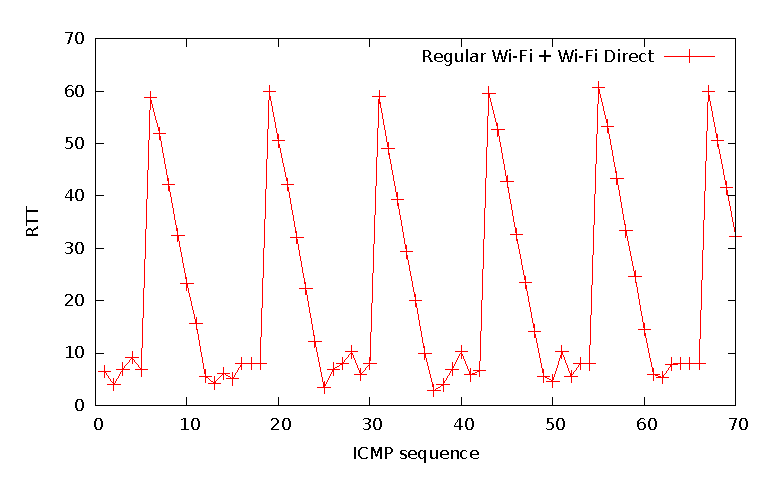
\includegraphics{src/img/regularwifi.eps}
\captionof{figure}{RTT for the Regular Wi-Fi Path}
\label{img:regular-wifi}
\end{figure}

\begin{figure}[h!]
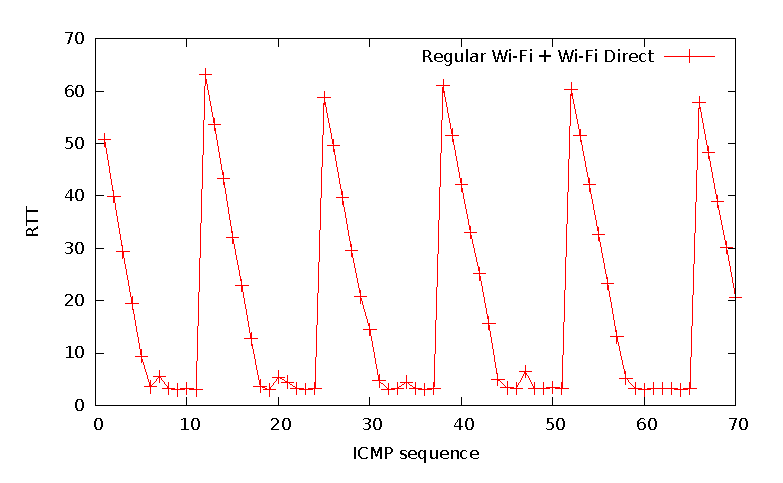
\includegraphics{src/img/wifidirectping.eps}
\captionof{figure}{RTT for the Wi-Fi Direct Path}
\label{img:wifi-direct}
\end{figure}

When the channel switching algorithm does not run, the average RTT value is very low, with an average RTT value at around 5 ms. For example, Figure \ref{img:regularwifionly} shows the RTT value for the case when we have just a regular Wi-Fi connection. The situation is the same for the Wi-Fi Direct only connection.

\begin{figure}[h!]
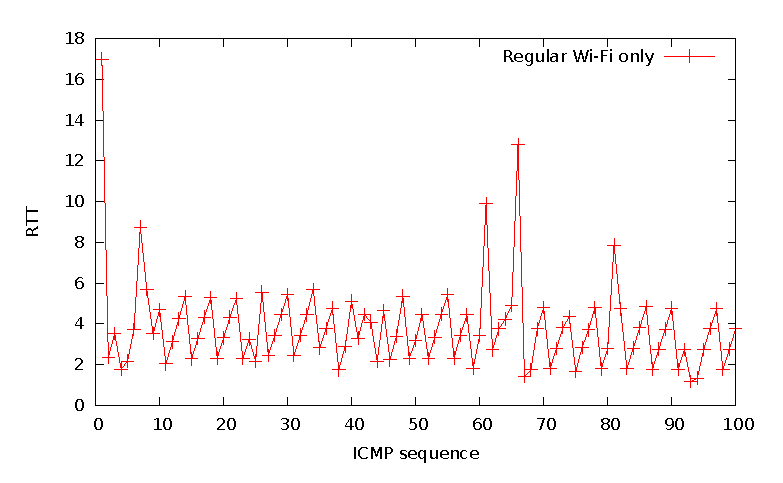
\includegraphics{src/img/regularwifionly.eps}
\captionof{figure}{RTT for the Regular Wi-Fi Path}
\label{img:regularwifionly}
\end{figure}

\newpage
\subsection{Channel-Switching Overhead}
\label{sub-sec:chsw-overhead}

The Channel Switch Overhead is the percent of time needed by the hardware to switch between two frequencies and no data can be transmitted or received during this switch. The idea of this test is to determine the maximum capacity of both paths by generating UDP packets with iperf in a single wifi scenario and getting the throughput value reported by iperf. Then, send UDP packets on both paths in a multiple wireless connectivity scenario with iperf and again get the throughput value. In an ideal case, if there is no channel switch overhead, the ratio between the throughput in a single wifi scenario and the throughput in a multi wifi scenario should be 2 for each channel.

For the Regular Wi-Fi path, the channel capacity is  about 230 Mbits/s. This value was obtained by generating UDP traffic from 192.168.0.101 towards 192.168.0.100. For the Wi-Fi Direct Path the channel capacity is about 55Mbits/s. This value was obtained by generated UDP traffic from the P2P-GO towards the P2P-Client.

The next step was to generate traffic on both paths in parallel. The iperf client used the maximum capacity of a path as parameter for bandwidth. The iperf server run on the P2P-client.

\begin{figure}[h!]
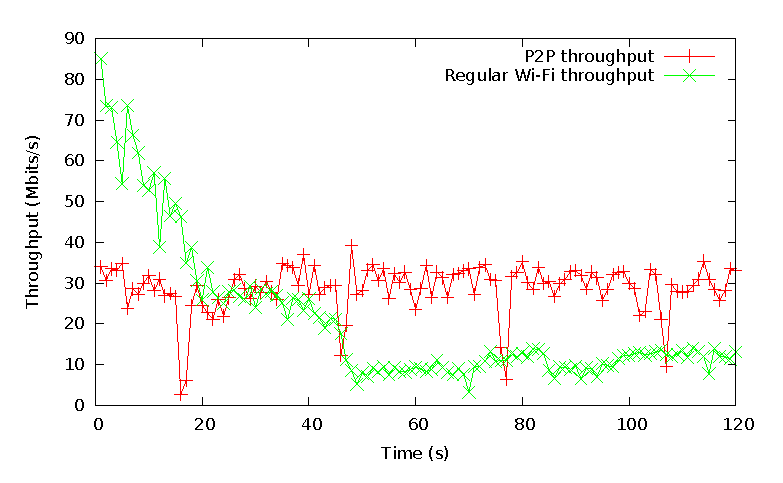
\includegraphics{src/img/throughpout.eps}
\captionof{figure}{UDP traffic for both paths, in parallel}
\label{img-thr}
\end{figure}

As can be seen in Figure \ref{img-thr}, the P2P throughput value is pretty stable and is about 30 Mbits/s. What is strange is that the throughput value for Regular Wi-Fi drops from about 85 Mbits/s to about 5 Mbits/s and this indicates an implementation bug in the channel switch algorithm. In order to determine the channel switch overhead, we can assume that the throughput for Regular Wi-Fi can maintain its value at 85Mbits/s. So the overhead is (1 - ((85 + 30) / (230 + 55) / 2)) * 100, which means that about 19\% of time is lost with the channel switching.

\newpage
\section{Average Power Tests - Channel Switching}
\label{sec:nexus5-consumption}

First of all we stopped all the running applications that came by default with the Nexus 5 devices. Then we measured the average power for 120s and made sure that there are no power spikes generated by an unwanted application. The average power in this case was 9.37mW.

For the next experiments we wanted to measure the energy consumption for different type of downloads. The steps are the following:
\begin{itemize}
  \item connect to the phone using the USB cable (adb shell).
  \item start an iperf instance: iperf -s -u -i 1 >> results_file \&\& nohup\&. Using this command we'll open a socket listening for UDP connections and the throughput results will be written in results file. The nohup command allows the iperf instance to run after we disconnect the USB cable.
  \item disconnect the USB cable.
  \item on the laptop start a long lasting UDP connection: iperf -c PHONE_IP_ADDRESS -u -t 6000 -i 1
  \item after the client iperf connection started, push the “RUN” button in the Monsoon device that will start gather consumption statistics.
  \item after Monsoon gathered results for 120 seconds, press “STOP” button in the Monsoon Software and save the results: the consumption file resulted from Monsoon and the results file from the phone where we have throughput.
\end{itemize}

\newpage
\subsection{Phone connected only to the AP}
\label{sub-sec:ap-only}
The average power for 120s when the phone is connected just to the AP but no data is transferred is 60.57mW. This value should be lower but it seems that some IPV6 Router Advertisements messages introduce some spikes in the power consumption graph from \labelindexref{Figure}{img:ap-only}. The blue line represents the average power, the red line represents the
minimum power and the green one represents the maximum power.

\fig[scale=0.5]{src/img/aponly.png}{img:ap-only}{Power when the phone is connected just to the AP}

\subsection{Phone connected in parallel to the AP and to the P2P GO}
\label{sub-sec:app2p-parallel}
In this case the average power consumption for 120s is 441.36mW. This value is correct as I repeated the experiments and the results are consistent.

\fig[scale=0.8]{src/img/app2pbis.png}{img:ap-p2p}{Power when the phone is connected in parallel to AP and to the P2P-GO}

\subsection{Data transfer using the Regular Wi-Fi connection, P2P connection only active}
\label{sub-sec:transfer-parallel}

In this experiment, the average power consumption for combined regular Wi-Fi + Wi-Fi Direct is compared with the average power consumption for regular Wi-Fi when we use the same throughput values. For this experiments, the Wi-Fi Direct connection is not used for data transfer, just an active connection between the P2P client and the P2P GO is kept alive. 

Detailed steps for the experiment are illustrated next. For x in (2.5, 5, 7.5, 10 Mbits/s) do:
\begin{itemize}
  \item connect the phone both to the AP and to the P2P GO
  \item on the phone start the iperf server to listen for new connections on the interface corresponding to the AP
  \item on the laptop generate traffic towards the client (iperf -c 192.168.0.100 -b x)
  \item calculate the average throughput value using the statistics file from the phone and save this average value (call it y)
  \item save the y value and the associated power average value
\end{itemize}

The results are:

\begin{table}[h!]
  \centering
  \caption{Power Monitor measurements (P2P + Regular Wi-Fi)}
  \label{tab:table1}
  \begin{tabular}{ccc}
    \toprule
    Throughput (Mbits/s) & Average Power (mW) \\
    \midrule
    2.49 & 472.8\\
    4.99 & 512.67\\
    7.48 & 547.66\\
    9.89 & 583.29\\
    \bottomrule
  \end{tabular}
\end{table}

\begin{itemize}
  \item connect the phone phone just to the AP
  \item on the phone start the iperf server
  \item on the laptop generate traffic towards the client (iperf -c IP_ADDR_PHONE -b y)
  \item On the client calculate the average throughput and save this average value
\end{itemize}

The results are:

\begin{table}[h!]
  \centering
  \caption{Power Monitor measurements (Regular Wi-Fi only)}
  \label{tab:table1}
  \begin{tabular}{ccc}
    \toprule
    Throughput (Mbits/s) & Average Power (mW) \\
    \midrule
    2.49 & 573.29\\
    4.99 & 634.14\\
    7.48 & 671.45\\
    9.89 & 752.45\\
    \bottomrule
  \end{tabular}
\end{table}

\begin{figure}
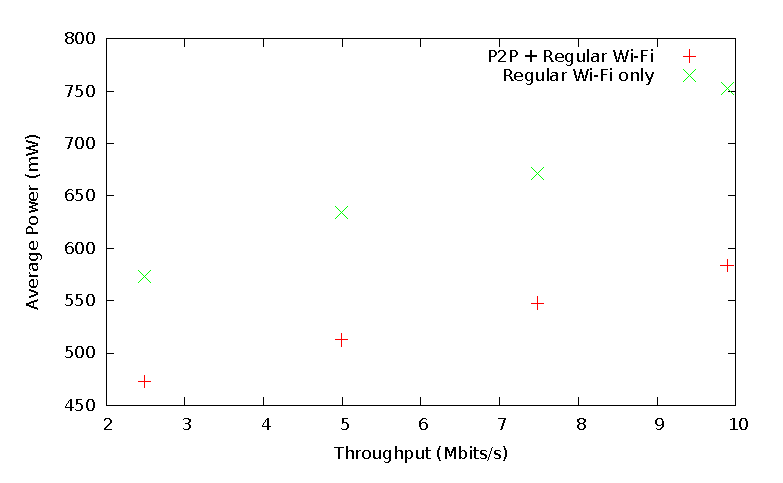
\includegraphics{src/img/powervalues.eps}
\captionof{figure}{Average Power for 120 seconds}
\end{figure}

It seems that by simply enabling the Wi-Fi Direct connection we get a power consumption improvement. We repeated the experiments several times and the results are consistent. This improvement could be explained by the batching mode of 802.11 where several packets are aggregated in a single, larger one. While the phone is on the Wi-Fi Direct channel, the packets are aggregated by the AP on the Regular Wi-Fi connection. When the client switches again on the Regular Wi-Fi connection, the larger packets are transmitted faster and more energy is saved.

\subsection{Data transfer using both the Regular Wi-Fi connection and the P2P connection}
\label{sub-sec:transfer-parallel2}

In this experiment, the average power consumption for combined regular Wi-Fi + Wi-Fi Direct was compared with the average power consumption for regular Wi-Fi when the same throughput values are used. Both the regular Wi-Fi and the Wi-Fi Direct connections were used for data transfer.

\begin{itemize}
  \item connect the phone both to the AP and to the P2P GO
  \item on the phone start 2 iperf server instances: one that listen for new connections on the interface corresponding to the AP and one that listen for new connection on the interface corresponding to the Wi-Fi Direct interface
  \item on the laptop generate traffic towards the client (iperf -c 192.168.0.100 -b x, iperf -c 192.168.49.1 -b x)
  \item calculate the combined average throughput value using the statistics file from the phone and save this average value (call it y)
  \item save the y value and the associated power average value 
\end{itemize}

The results are:

\begin{table}[h!]
  \centering
  \caption{Power Monitor measurements (Regular Wi-Fi + P2P parallel transfer)}
  \label{tab:table1}
  \begin{tabular}{ccc}
    \toprule
    Throughput (Mbits/s) & Average Power (mW) \\
    \midrule
     4.99 & 472.8 \\
     9.96 & 575.67 \\
     14.5 & 685.19\\
     19.05 & 742.89 \\
    \bottomrule
  \end{tabular}
\end{table}

\begin{itemize}
  \item connect the phone phone just to the AP
  \item on the phone start the iperf server
  \item on the laptop generate traffic towards the client (iperf -c 192.168.0.100 -b y)
  \item on the client calculate the average throughput and save this average value
\end{itemize}

The results are:

\begin{table}[h!]
  \centering
  \caption{Power Monitor measurements (Regular Wi-Fi transfer only)}
  \label{tab:table1}
  \begin{tabular}{ccc}
    \toprule
    Throughput (Mbits/s) & Average Power (mW) \\
    \midrule
     4.99 & 634.14 \\
     9.96 & 757.79 \\
     14.5 & 787.36 \\
     19.05 & 985.13 \\
    \bottomrule
  \end{tabular}
\end{table}

\begin{figure}[bp!]
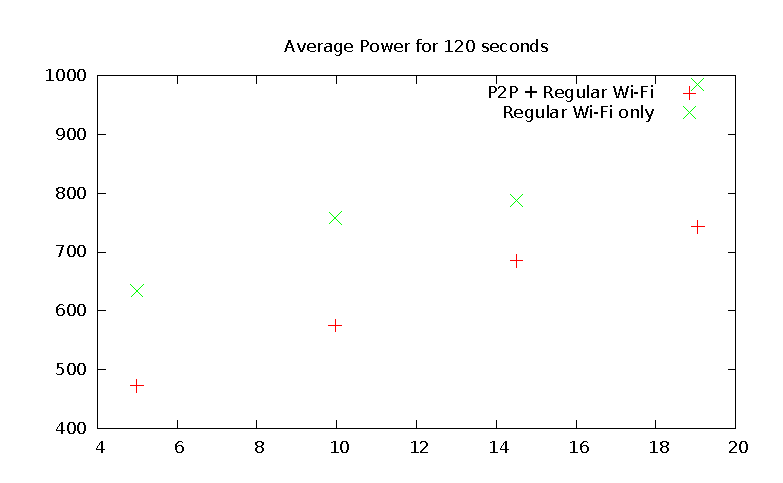
\includegraphics{src/img/powervaluesparallel.eps}
\captionof{figure}{Average Power for 120 seconds}
\end{figure}

Also In this case the power average values are better in case of regular Wi-Fi combined with Wi-Fi Direct.

\section{Average Power Tests - Single Channel}
\label{sec:nexus5-consumption}

For this test, both the Regular Wi-Fi and the Wi-Fi Direct connections are using the same 2.4 channel and no data is transferred, only the management frames. The average power for 120s is around 210mW. In this case no energy spikes are observed which demonstrates that there is no power saving scheme implemented.

\fig[scale=0.65]{src/img/app2psame.png}{img:ap-p2psame}{Power when the phone is connected in parallel to AP and to the P2P-GO}


\section{Power Management}
\label{sec:PowerManagement}

For understanding the multiple Wi-Fi connectivity on Nexus 5, traffic was generated using the ping command. An interesting behaviour occured when ICMP packets were generated at intervals greater than 500ms: once the screen was turned off no packets were put into the air. After analysing the Broadcom driver code, we found the root of this behaviour inside \textit{kernel/lge/hammerhead/drivers/net/wireless/bcmdhd/dhd.h}. The define \textit{DHD_PACKET_TIMEOUT_MS} is set to 500 which mean that if the ping interval is lower than this timeout, the ICMP packets are sent even when the screen is turned off, otherwise the ping activity is suspended and resumed only after the screen is on again. 

It proved that \textit{DHD_PACKET_TIMEOUT_MS} configures the timeout for a wakeup event which is the basis for the Android Power Management model. For a better understanding of this model, the original discussion from the mailing list \cite{cite-wakesdiscussion} is analysed.

The main task of the Android PM is first to verify that there are no pending wakeup events, then to freeze all user/kernel space processes and allow the device to go in suspend mode. Stated problems are related to the loss of wakeup events. First, if a wakeup event occurs exactly at the same time when /sys/power/state is being written to, the event may be delievered to user space right before the freezing of it in which case the space consumer of the veent may not be able to process it before the system is suspended. Second, if a wakeup event occurs after user space has been frozen and that event is not a wakeup interrupt, the kernel will not react to it and the system will be suspended.

The sys interface for PM management is:
\begin{itemize}
  \item /sys/power/state - write "mem" to enter suspend mode
  \item /sys/power/wakeup_count - counter of wakeup events. This value will be read in the kernel code base and verified if equal or not to an interval counter. This check is done to know if the device can enter or not in suspend ode and write in /sys/power/state. May be read from or written to by user space. Reads will always succeed and return the current value of the wakeup events counter. Writes, however, will only succeed if the written number is equal to the current value of the wakeup events counter. If a write is successful, it will cause the kernel to save the current value of the wakeup events counter and to compare the saved number with the current value of the counter at certain points of the subsequent (or hibernate) sequence. If the two values don't match, the suspend will be aborted just as though a wakeup interrupt happened. Reading from /sys/power/wakeup_count again will turn that mechanism off;
\end{itemize}

The Android PM is a user-space process that that will first read from /sys/power/wakeup_count. Then it will check all user space consumers of wakeup events known to it for unprocessed events. If there are any, it will wait for then to be processed and repeat. In turn, if there are not any, it will try to write to /sys/power/wakeup_count and if the write is successful, it will write to /sys/power/state to start suspend, so if any wakeup events occur past that point, they will be noticed by the kernel and will eventually cause the suspend to be aborted.

Drivers and kernel subsystems can signal wakeup events. If the event is not explicitly handed over to user space and "instantaneous", they can simply call \textit{pm_wakeup_event()} and be done with it. Second, if the event is going to be delivered to user space, the subsystem that processes the event can call pm_wakeup_begin() right when the event is detected and pm_wakeup_end() when it's been handed over to user space. \textit{pm_get_wakeup_count()} and \textit{pm_save_wakeup_count()} fail if they are called when events_in_progress is nonzero. For pm_save_wakeup_count() that's pretty obvious (I think) and it also kind of makes sense for pm_get_wakeup_count(), because that will tell the reader of /sys/power/wakeup_count that the value is going to change immediately so it should really try again.”;

One possible problem that can still appear in PM is that processes can be frozen before an event is handled by the kernel. For example and interrupt handler might receive the event and start processing it by calling \textit {pm_request_resume} - but if the PM workqueue thread is already frozen then the processing won't finish until something else wakes the system up.

The codebase for this analysis is represented by:
\begin{itemize}
  \item kernel/lge/hammerhead/drivers/net/wireless/bcmdhd
  \item kernel/lge/hammerhead/drivers/base/power
  \item kernel/lge/hammerhead/kernel/power
  \item system/core/libsuspend
  \item sysfs
\end{itemize}

\section{Conclusions}
\label{sec:conclusions}

The implementation for multiple Wireless Connectivity on Android has multiple problems. Both for Single and Multiple Channel Connectivity, there is no power save algorithm implemented and the Wi-Fi card enters a high energy-mode once the second connection is established. Also, the channel swirching algorithm is pretty rudimentary because the channel switching quantum is the same with no load-balancing depending on the traffic pattern. 

Unfortunately, no improvements could be done to this algorithm as the code for it is in the Broadcom closed-source firmware. The next step was to find a smartphone whose firmware code for Wi-Fi is open-source but it seems that all implementations are proprietary solutions.

\chapter{Power-Save Algorithm for Multiple Wireless Connectivity}

As shown in the previous chapter, the first step for implementing a power save algorithm for multiple wireless connectivity is an open-source firmware. In most of the cases this also implies an open-source hardware described by a datasheet. This is due to the fact that the firmware code works directly with the Wi-Fi card registers.

Currently, there is no smartphone whose firmware is open-source for the Wi-Fi card so the work-around was to use an Wi-Fi dongle, a TP-Link TL-WN722N card \cite{cite-tplink} who is totally open-source. This chapter starts with the challenges in using this dongle with Nexus 5, it continues with an analysis of the open-source firwmare and it presents our algorithm for Power Save implemented on top of this platform.

\section{Using the Wi-Fi dongle with Nexus 5}
\label{sec:donglesmartphone}

The micro-USB port of the smartphone was used for connecting the Wi-Fi dongle, as can be observed in \labelindexref{Figure}{img:dongle-wifi}. The driver used by the dongle is ath9k_htc so we had to enable loadable module support plus ath9k_htc in the kernel menuconfig. However there was an 'Exec format' error while trying to insert the ath9k_htc.ko module using the insmod shell command. The insmod command calls in the bacground the init_module system call:

\begin{lstlisting}[language=C, frame=single, caption={init_module system call},label=InterfaceCombinations]
int init_module(void *module_image, unsigned long len, const char *param_values);
\end{lstlisting}

\fig[scale=0.2]{src/img/nexus5kali.jpg}{img:dongle-wifi}{Wi-Fi dongle connected to Nexus 5}

The role of the init_module is to load an ELF image into kernel space, perform the necessary relocations and initializations then run the module's init function. This functions receives third parameters: the module_image argument points to a buffer containing the binary image to be loaded; len specifies the size of that buffer and the param_values is a sting containing space-delimited specifications of the values for module parameters. In our case, there was a problem in the busybox implementation for insmod: the second argument was 8 bytes long instead of 4. When the init_modules was looking for the parameters passed on the stack and was trying to parse the third parameter it would actually look in the last 4 bytes of the second parameter, which were all zeros in most of the cases. So the third parameter was NULL in most of the cases. Later, in kernel space when SYSCALL_DEFINE3 is caled with a NULL parameter, the -EFAULT error is set. The solution was to use a 4 byte long parameter for the len argument.

\subsection{Measuring the energy consumption for the Wi-Fi Dongle}
\label{sec:dongleenergy}

The chipset mounted inside the TP-Link dongle is AR9271. Both the firmware \cite{cite-firmware} and the datasheet are open-source. In order to avoid the noise introduced by the phone components and by the USB layer, our first approach was to measure the energy consumption of the AR9271 chipset only. If we could find an entry point for the current in the AR9271 chip then we could easily use the AUX port of the power monitor device. This port allows for simultaneous measurement of the current going through an external power supply by using a sense resistor with a very low resistance (0.1 ohm) and a bayonet Neill-Concelman (BNC) connector.

AR9271 has 68 pins and the datasheet states that pins 17, 26, 33,47 represents digital 3.3 V power supply - VDDP33. Having multiple 3.3V power supply pins is common practice because it allows the PCB designer to create better PCBs in terms of RF immunity, RF emissions and signal crosstalk. 

\fig[scale=0.3]{src/img/donglefront.jpg}{img:dongle-front}{A9271 subsystem from TP-Link WN7222N}

However, the power monitor device has a single grabber for IN current so a common entry point for these multiple 3.3V pins was was needed. Although the datasheet for the AR9271 chip is open-source, the datasheet for the entire TP-Link Dongle is closed-source. \labelindexref{Figure}{img:dongle-front} shows the circuit around the AR9271 chip and it seems that the solution to the above problem would be to intercept the 3.3V rail after the step down converter, the trace right after 4R7, highlighted with red. Probably, the power consumption parameters from section 6.9 o f the datasheet were gathered using this technique. More details about this discussion can be found at \cite{cite-ar9271} 

Because the above assumptions were not backed-up by a datasheet we decided that is safer to measure the power consumption of the entire USB dongle. This was achieved by using the USB channel of the power monitor that offers the possibility to intercept the connection between the Wi-Fi Dongle and a USB port. More exactly, on the Power Monitor device are two ports: an USB type A port and a USB type B port. The Wi-Fi dongle was plugged-in the USB type A port, while the the laptop is connected to the USB type B port. The Monsoon Software offers the possibility to monitor this  USB channel.

To download code or data when testing a device, USB can be used to connect the device to
the Mobile Device Power Monitor. However, when connecting to USB, USB charges the
device, which disturbs the current measurements. To remedy this, the Mobile Device Power
Monitor has an Auto USB passthrough mode. Auto USB passthrough mode is useful
for testing, because in Auto USB passthrough mode, the USB pass-through is
disconnected whenever sampling starts. After sampling has completed, USB is reconnected
automatically so that test data can be loaded to the device. The Auto USB passthrough
mode setting is shown in below in \labelindexref{Figure}{img:usb-controls}.

This technique proved to be useful because the graphic for the avergage power when no data is transmitted/received is constant and we were able to see the traffic spikes generated when by the AR9271 enters/exit sleep mode.

\fig[scale=1]{src/img/usbm.png}{img:usb-controls}{Options for USB channel monitoring}

\subsection{Firmware Debugging for the Wi-Fi Dongle}
\label{sec:firmwaredebugging}

The AR9271 is a USB/Wifi SoC with onboad RAM, ROM, flash and the actual wireless chip.  The wireless core is an off-shoot of the AR9285, a single-chip solution. For firmware debugging, the AR9271 chip has 16 GPIO pins and some of them can be configured to work in UART mode.  Gathering data from these pins is done using a TTL UART adapter. For example, the operating system running on the SoC offers the possibility to print the value of variables.

Our first approach was to solder the TX/RX wires of the TTL UART directly to the GPIO pins of the AR9271 chip from the TP-Link Dongle. Unfortuntely, the distance between two nearby pins is very small and we didn't have specialized soldering equipment. The solution was to use another dongle, a ALFA Network AWUS036NHA which uses the same AR9271 chip but has accesible UART lines on the PCB. This setup is illustrated in \labelindexref{Figure}{img:ttl-uart}.

\fig[scale=0.12]{src/img/ttl.jpg}{img:ttl-uart}{TTL UART connected to AWUS036NHA dongle}

\section{Starting point for the algorithm}
\label{sec:fix}

PS Algorithm for multiple wireless interface is based on the ath9k_htc standard PS algorithm. The problem is that PS support for ath9k_htc driver is buggy: RX wake-up is not properly implemented. When there is no data transmitted, the WiFi card is put to sleep. The WiFi card enters the 'NETWORK SLEEP' state where the MAC subsystem is in low-power mode and no data is received from the AP that the client is associated to. The RTC subsystem is always on and can be programmed to wake up periodically the MAC subsystem (e.g.: for BEACONs with DTIM set). Using the hardware timers represented by MAC_PCU_SLP1 and MAC_PCU_SLP2 registers, the card can be programmed to wake up periodically for management frames. The problem is that the current implementation does not correctly program these hardware timers and the hardware is woken up by software timers instead or by TX operations:
\begin{itemize}
\item there is a mac80211 software timer that detects 7 beacon lost and wake up the card
\item mac80211 wakes up the hardware when there is a new frame for TX.
\end{itemize}

The above bug can be easily reproduced if the Wi-Fi dongle is connected to an Access Point then power save mode is enabled without generating any traffic. According to the IEEE802.11 specification, the card should wake up for RX traffic at least at DTIM intervals. In our setup, the AP has a configured DTIM of 100ms. \labelindexref{Figure}{img:ps-single} illustrates the power pattern of the Wi-Fi dongle with the above setup. Delta time between cursors is 795 ms. This time corresponds with the timeout for mac80211 software timer reponsible for beacon loss (ieee80211_mgd_probe_ap).

NEXT_DTIM is the timer responsible for waking up the card at each DTIM interval. ath9k_htc driver correctly sets up this timer by setting up its two parameters: when it should arm for the first time and the period of this timer. However, it seems that the timer is triggered just a single time and the period parameter of the trigger is ignored. The solution was to rearm the timer each time a new beacon is received from the AP. \labelindexref{Figure}{img:ps-single} illustrates the power save capture after bug resolution and it can be observed that the card wakes up at each DTIM interval. This time, delta time between cursors is about 100 ms. More details can be found at \cite{cite-wikisingleps}.

\fig[scale=0.45]{src/img/pssingle.png}{img:ps-single}{Power capture during Power Save bug}
\fig[scale=0.45]{src/img/psoksingle.png}{img:ps-single}{Power capture after bug resolution}

\clearpage
\section{Double wake-up algorithm}
\label{sec:twowakeup}

ath9k_htc does not have PS support for multiple interfaces. Once the second virtual interface is created, PS is automatically disabled and the card is always in the awake state with an averge power of about 600mW.

\fig[scale=0.45]{src/img/awakestate.png}{img:mps-single}{Power capture with no PS support}

The power save algorithm that I implemented is split in two sections, a mac80211 section and an ath9k_htc section. At this moment the algorithm is limited to a maximum of two virtual interfaces and the the DTIM periods for the AP has to be equal.

The mac80211 generic section is responsible for sending the NULL frames. Behaviour:
\begin{itemize}
\item when the STA received a directed TIM for one of the virtual interfaces it will send 2 NULL functions with the PS bit set, one on each interface. Most of the modifications were done in ieee80211_rx_mgmt_beacon;
\item a single timer (ieee80211_dynamic_ps_timer) schedules the tasklet for enabling PS. Timeout for this timer expires when no data is sent on any interface.
\item when the tasklet for enabling PS mode is scheduled (ieee80211_dynamic_ps_enable_work) it will first send 2 NULL functions with the PS bit unset, one on each interface. After both NULL frames are ACK'ed, mac80211 requests the driver to put the chip in sleep mode. 
\end{itemize}

The ath9k_htc part of the PS algorithm is responsible for waking up the card for RX traffic. This time, we have to wake up the hardware at DTIM periods which corresponds to DTIM periods for each AP that the chip is connected to. Let's assume that the dongle is connected at two APs, AP1 and AP2, each AP with the same dtim period, DTIM_PERIOD. The algorithm starts with the card in the awake state. The card will first capture one beacon from AP1 and it will save a value equal with the current time + DTIM_PERIOD. Then, the card will capture a beacon from AP2, it will arm the NEXT_DTIM timer with the saved valued and the saved value is replaces with a value equal with the current time + NEXT_DTIM. At this moment the card can enter power save mode. When it will wake up due to NEXT_DTIM timer, the NEXT_DTIM timer is re-armed wth the saved value and the saved value is replaced with the current_time + DTIM_PERIOD.

For a better granularity of the timers, the current time was replaced with the value read from the LAST_TSTP register, which gives the timestamp of the last beacon received. The problem is that this register is updated with the last timestamp of the beacon received from the AP that we first established a connection with. 

The algorithm behaves as expected until one random point when the card exists unexpectedly from power save. According to Wireshark captures, the algorithm still sends NULL frames correctly on both paths but the power monitor capture shows that the card enters the awake state. A discussion was started with Qualcomm developers, \cite{cite-bugps}, but no solution was found yet.

\section{Single wake-up algorithm}
\label{sec:singlewakeup}

A disadvantage of the double wake-up algorithm is the fact that the card has to stay awake most of the time as the number of the interfaces increases even if there is only management traffic (beacons). This is due the fact that the hardware has to wake up to capture DTIM beacons for each AP and if there is no traffic go back to sleep again. As the number of the APs that we are connected to increases there is a high probability that the delta time between waking up for DTIM beacons for two different APs to be very short. It's true that the RTT will be very short as the client can drain quickly buffered packets but the energy saving will be minimal.

The idea of the single wake-up algorithm is to use NEXT_DTIM timer only for the first AP that the client connected to, just as is done in the standard implementation then add the following modifications for multiple interface power save: 

\begin{itemize}
\item when the card wakes up due to NEXT_DTIM timer expiration, send NULL frames with the PS bit unset to all the other APs that the client is connected signaling them that sending of the buffered frames is allowed. According to the IEEE802.11 specification for Power Save, AP can send buffered frames once it received the NULL frame with PS=0 from a client;
\item if no traffic is received from any of the APs for more than a configurable mac80211 timeout, then enter PS mode by send NULL frames with PS bit set to all the APs that the client is connected to. 
\end{itemize}





